\documentclass{article}
\usepackage{booktabs}
\usepackage{arydshln}
\usepackage{sectsty}
\usepackage{geometry}
\usepackage{float}
\usepackage{url}
\usepackage{titlesec}
\usepackage{amssymb}
\usepackage{fancyhdr}
\usepackage{setspace}
\usepackage[italian]{babel}
\usepackage{graphicx} % Required for inserting images
\usepackage{caption}
\usepackage{subcaption} % Required for subcaptions
\usepackage{titling}
\usepackage{tikz}
\usepackage{varwidth} % Required for centering the title
\usepackage{datetime2} % Required for custom date format
\usepackage{hyperref}
\usepackage{tocloft}
\renewcommand{\cftsecfont}{\boldmath\Large}
\renewcommand{\cftsubsecfont}{\boldmath\large}
\renewcommand{\cfttoctitlefont}{\LARGE\boldmath\bfseries} % Dimensione e stile del titolo dell'indice
\renewcommand{\cftsecfont}{\bfseries\boldmath\Large} % Sezioni principali con grassetto più forte
\renewcommand{\cftsubsecfont}{\large} % Sottosezioni non in grassetto

\sectionfont{\LARGE}
\subsectionfont{\Large}
\sectionfont{\fontsize{22}{24}\selectfont\bfseries}
\setstretch{1.2} % Regola lo spaziamento tra le righe dei paragrafi
\setlength{\parindent}{0pt} % Rimuove l'indentazione dei paragrafi
\titleformat{\section}{\fontsize{16}{18}\selectfont\bfseries}{\thesection}{1em}{}

\geometry{
  left=3.5cm,
  right=3.5cm,
  top=3.5cm,
  bottom=3.5cm,
}

\hypersetup{
    linktoc=all,
    linkbordercolor=white, % Imposta il colore del bordo dei link a bianco
    colorlinks=true,
    linkcolor=black,
    urlcolor=cyan,
    pdftitle={Esercizio A: coda con priorità},
}


\begin{document}

\pagestyle{fancy}
\fancyhf{}
\rhead{\thepage}

\begin{titlepage}
    \centering
    
    
\includegraphics[width=1\textwidth]{Images/LogoUnifi.png}
    
    \captionsetup[figure]{labelformat=empty}
    \captionof{figure}{\fontsize{16}{24}\selectfont Università degli studi di Firenze}
    
    \vspace{2cm}
    
    \begin{center}
      \Huge\bfseries\fbox{\begin{varwidth}{\dimexpr\linewidth-20pt} % Increase the padding to 20pt
      \centering LABORATORIO DI ALGORITMI E STRUTTURE DATI
      \end{varwidth}}
    \end{center}
    
    \vspace{2cm}
    
    {\Large\bfseries Autore:} {\Large Ivan Necerini} \\
    {\Large\bfseries Numero di matricola:} {\Large 7049380} \\
    {\Large\bfseries Corso principale:} {\Large Algoritmi e strutture dati} \\
    {\Large\bfseries Docente:} {\Large Simone Marinai}
    
    \vfill
    
    May 2023
    
\end{titlepage}

\tableofcontents

\clearpage

\titleformat{\section}[display]
  {\normalfont\Large\bfseries}
  {}
  {0pt}
  {}
\titlespacing*{\section}
  {0pt}
  {0pt}
  {0pt}

\titleformat{\section}[hang]{\normalfont\Large\bfseries}{\thesection}{1em}{\raggedright}
\titleformat{\subsection}[hang]{\normalfont\large\bfseries}{\thesubsection}{1em}{\raggedright}

\section{Introduzione}
Lo scopo della presente relazione è confrontare diverse implementazioni della coda con priorità. Sono state realizzate tre diverse strutture dati per implementare la coda con priorità: il \textbf{max heap}, la \textbf{lista concatenata} e la \textbf{lista concatenata ordinata}.

Verranno analizzate e confrontate le prestazioni delle operazioni di inserimento, ricerca del massimo ed estrazione del massimo, che sono le operazioni più significative, su una coda con priorità implementata utilizzando le tre diverse strutture dati menzionate in precedenza.

\subsection{Specifiche della piattaforma di test}
Il codice per eseguire gli esperimenti è stato scritto in Python (interprete v.3.10.2, ultima versione a oggi), utlizzando l'ambiente di sviluppo "Microsoft Visual Studio Code" v.1.78.2. 

Il computer su cui è stato scritto il codice ha le seguenti specifiche:

\begin{itemize}
  \item Processore 11th Gen Intel(R) Core(TM) i7-1165G7 @ 2.80GHz
  \item RAM installata 16,0 GB (15,8 GB utilizzabile)
  \item Sistema operativo a 64 bit, processore basato su x64
  \item Windows 11 Home Versione	22H2
\end{itemize}

La presente relazione è stata scritta in \LaTeX tramite l'editor online Overleaf.

Il diagramma delle classi in Figura \ref{fig: DiagrammaDelleClassi} è stato disegnato tramite il software Lucidchart.

\subsection{Librerie utilizzate}
Segue una lista delle librerie principali utilizzati nella scrittura del codice python:

\begin{itemize}
    \item \verb|numpy|: per generare array con valori casuali
    \par (funzioni usate: numpy.random.randint())

    \item \verb|os|: per creare le cartelle dove salvare le immagini di grafici e tabelle
    \par (funzioni usate: os.path.exists() e os.makedirs())

    \item \verb|sys|: utilizzata per aumentare il limite di ricorsione massimo, necessario per evitare che venga generato un errore di ricorsione
    \par (funzioni usate: sys.setrecursionlimit())

    \item \verb|anyTree|: offre strumenti per lavorare con alberi gerarchici, ovvero collezioni di nodi interconnessi da archi. La funzione Node() di anyTree crea un nuovo nodo con il nome specificato e l'aggiunge all'albero. La funzione RenderTree() restituisce una rappresentazione in stringa dell'albero con i nodi indentati in modo da riflettere la loro gerarchia.
    \par (funzioni usate: anyTree.Node() e anyTree.RenderTree())

    \item \verb|copy|: utilizzata per fare copie profonde di oggetti
    \par (funzioni usate: copy.deepcopy() )

    \item \verb|functools|: utilizzata per lavorare con funzioni di ordine superiore e oggetti chiamabili. La funzione 'partial' si usa poi per creare nuove funzioni parzialmente applicate a partire da una funzione esistente
    \par (funzioni usate: functools.partial() )

    \item \verb|timeit|: utilizzata per misurare i tempi di esecuzione degli algoritmi
    \par (funzioni usate: timeit.timeit(stmt, number))
    
    \item \verb|matplotlib|: utilizzata per generare grafici e tabelle in modo da vedere effettivamente le prestazioni degli algoritmi
    \par (funzioni usate: matplotlib.pyplot.plot() e matplotlib.pyplot.table())

\end{itemize}

\label{sec:usoLibrerie}

\clearpage

\section{Cenni teorici}
Una \textbf{coda con priorità} è una struttura dati utilizzata per gestire un insieme dinamico di elementi denominato "S". Ogni elemento in questa coda è associato a un valore chiamato "chiave", che determina la sua priorità. Nei nostri esperimenti, valori più alti di chiave indicano una priorità più elevata.

Le operazioni fondamentali per il corretto funzionamento e utilizzo della coda con priorità includono l'inserimento di elementi, la ricerca del valore massimo e la sua eventuale estrazione. In questa relazione, analizzeremo e confrontaremo queste operazioni nelle diverse implementazioni della coda con priorità.

\subsection{Schema delle classi, organizzazione del codice e delle strutture dati}
Il diagramma delle classi è rappresentato in figura \ref{fig: DiagrammaDelleClassi}, al fine di spiegare al meglio l'organizzazione del codice Python. 

\begin{figure}[h]
    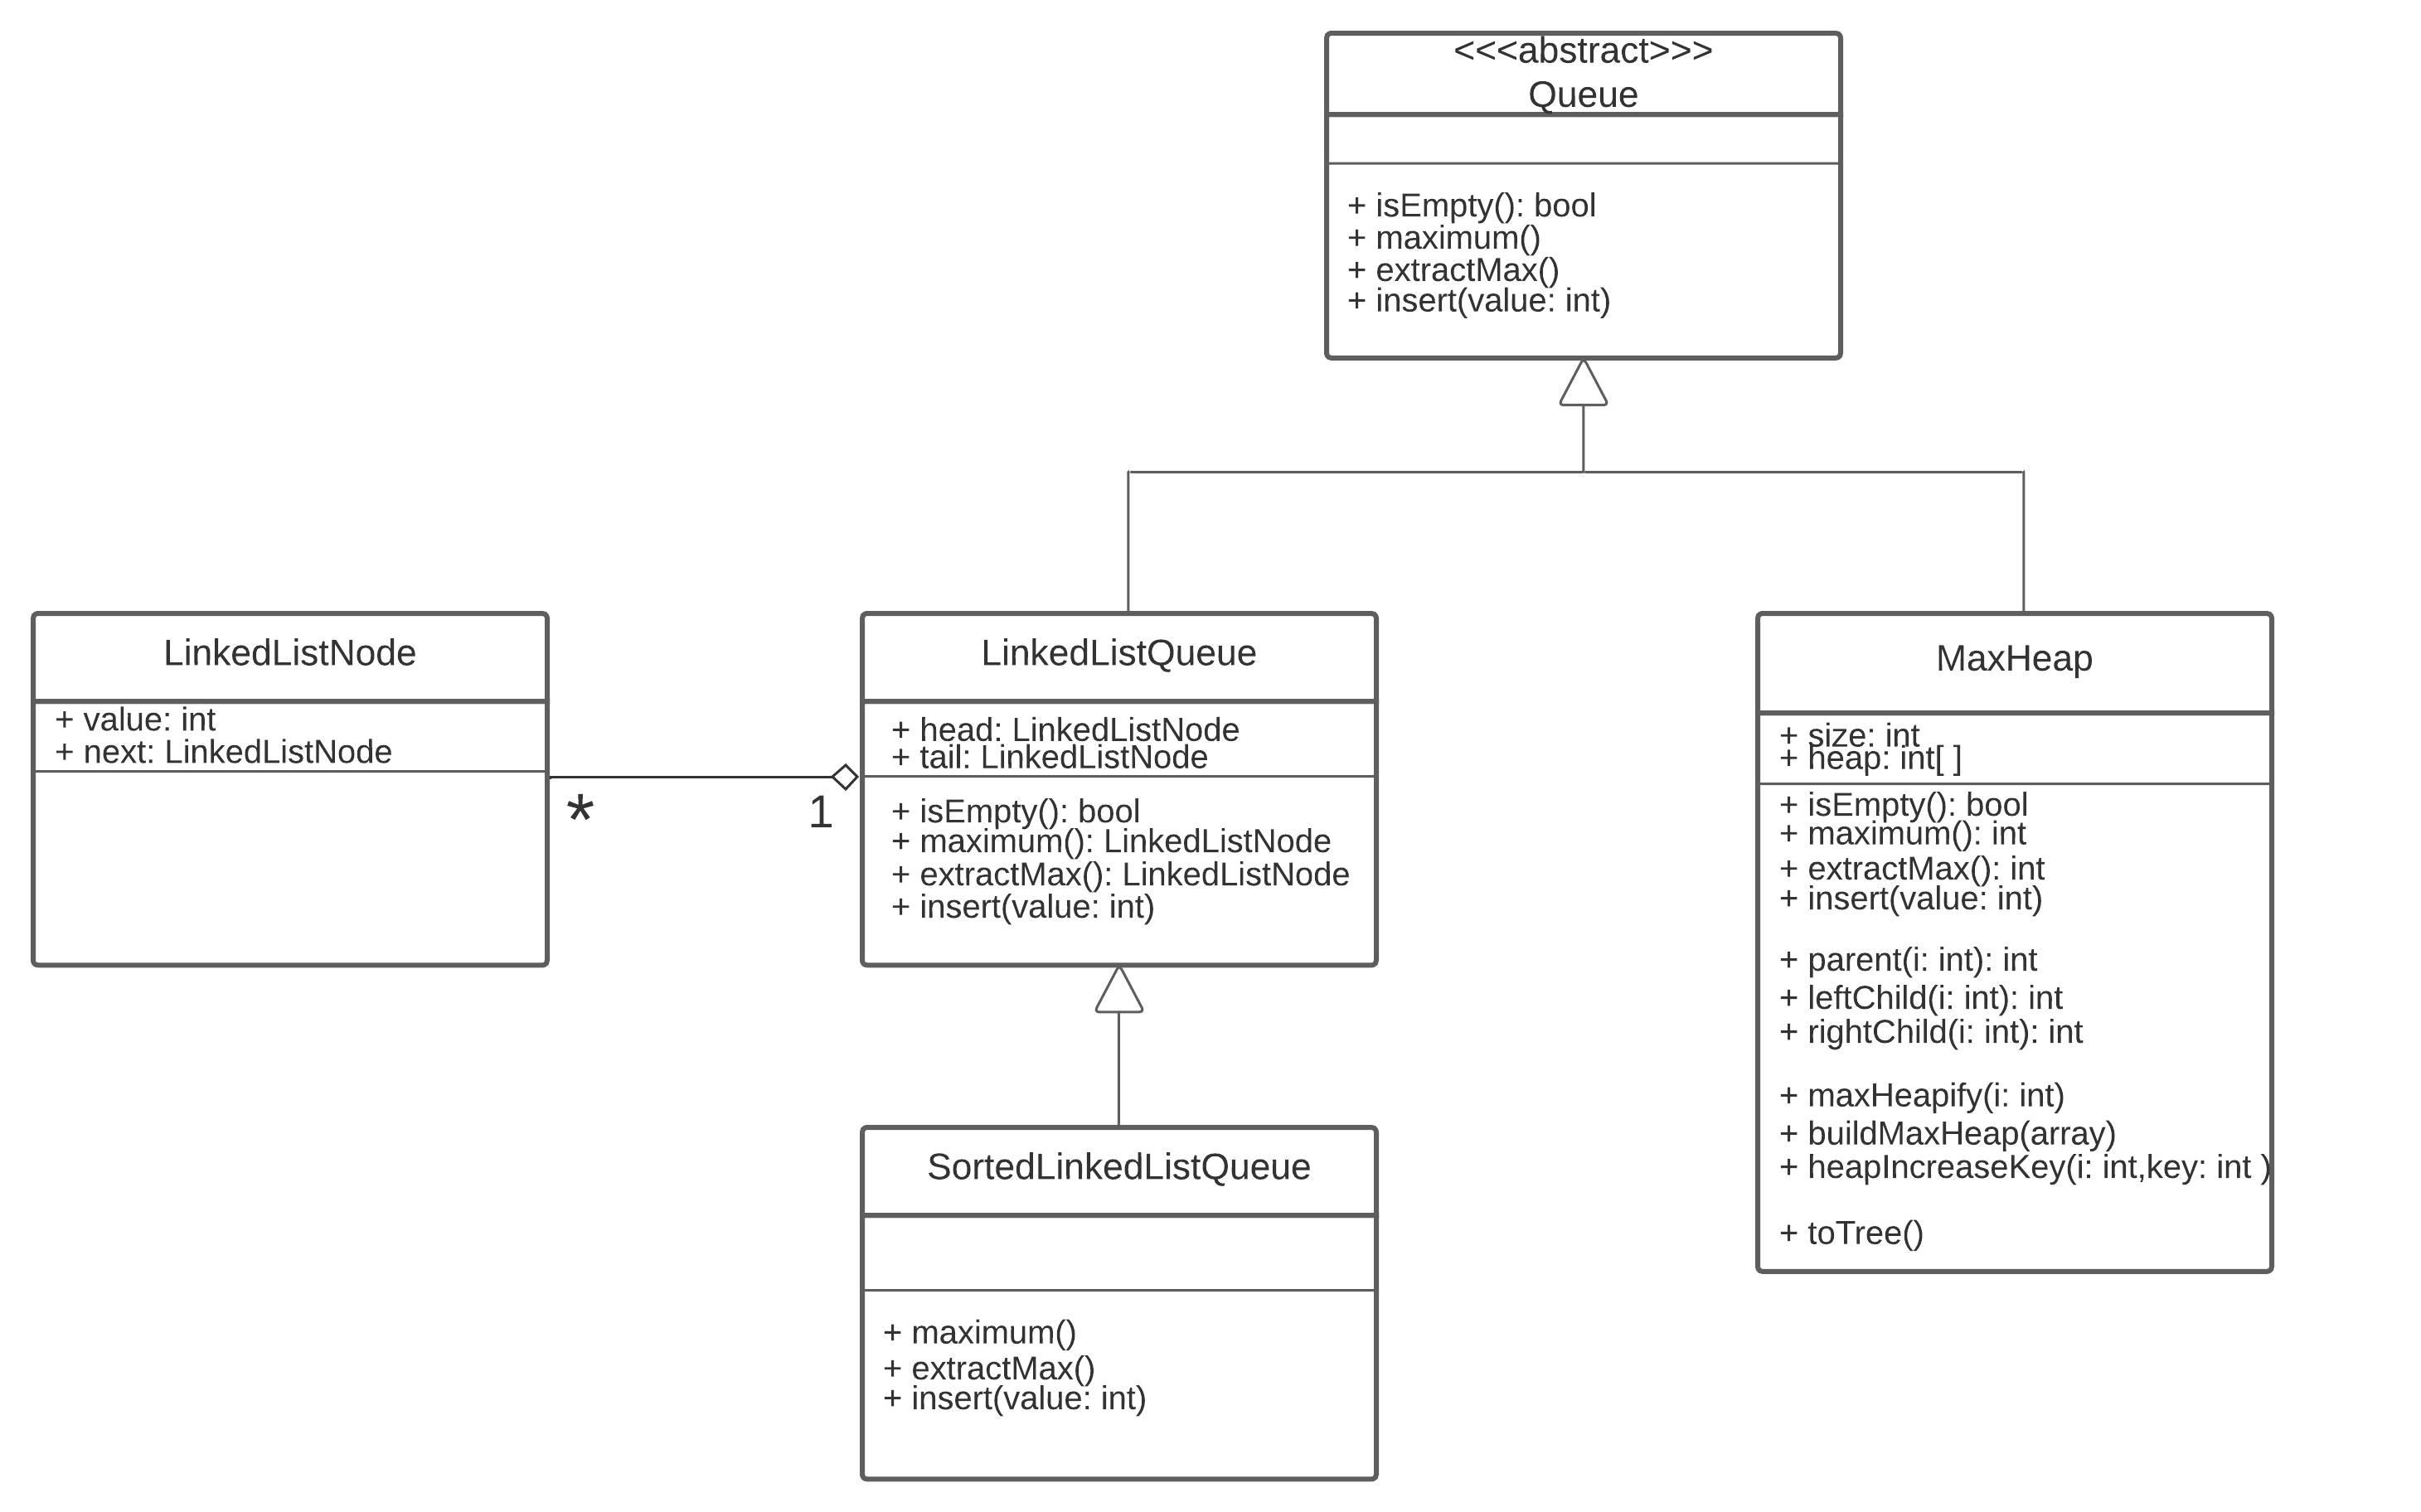
\includegraphics[width=1\textwidth]{Images/DiagrammaDelleClassi.png}
    \centering
    \caption{Diagramma delle classi}
    \label{fig: DiagrammaDelleClassi}
\end{figure}

La relazione ha lo scopo di condurre test su tre operazioni di una coda con priorità, implementata utilizzando diverse strutture dati. Per raggiungere questo obiettivo, è stata creata una classe astratta chiamata "Queue". La classe "Queue" contiene i prototipi dei metodi fondamentali per il corretto funzionamento di una coda con priorità. Ciò impone alle classi derivate (che sono concrete) di implementare effettivamente tali metodi, al fine di rendere la coda con priorità utilizzabile con le diverse strutture dati implementate.

\subsubsection{Max heap}
Un heap binario (classe \textit{MaxHeap} in figura \ref{fig: DiagrammaDelleClassi} è una struttura dati composta da un array che può essere considerato come un albero binario quasi completo (per questo mtoivo la sua altezza è di $\Theta(\log_2(n))$) come mostrato nella figura \ref{fig: Heap1}, dove il numero all'interno del cerchio è il valore registrato dentro quel nodo e il numero sopra è l'indice del corrsipondente array. Ogni nodo dell'albero corrisponde a un elemento dell'array che memorizza il valore del nodo. Tutti i livelli dell'albero sono completamente riempiti, tranne l'ultimo che potrebbe non essere completamente riempito dalla sinistra. Un array H che rappresenta un heap è un oggetto con due attributi: lunghezza[H] che indica il numero di elementi nell'array e size[H] che indica il numero di elementi dell'heap registrati nell'array H. In altre parole, anche se H[1...lunghezza[H]] contiene numeri validi, nessun elemento dopo H[size[H]], dove size[H] \(\leq\) lunghezza[H], è un elemento dell'heap.

\begin{figure}[H]
    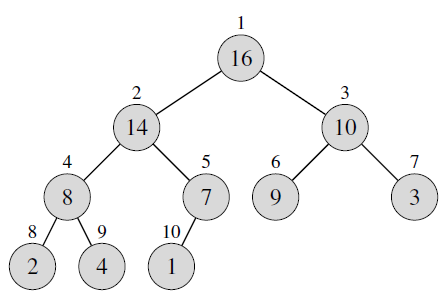
\includegraphics[width=0.6\textwidth]{Images/Heap1.png}
    \centering
    \caption{MaxHeap visto come un albero binario}
    \label{fig: Heap1}
\end{figure}

\footnote{Fonte dell'immagine: \textit{Introduzione agli algoritmi e strutture dati}, pagina 128, Cormen, Leiserson, Rivest e Stein, \emph{McGrawHill}, 2010.}

Ci sono due tipi di heap binari: maxHeap e minHeap. In entrambi i valori nei nodi soddisfano una proprietà dell'heap, le cui caratteristiche dipendono dal tipo di heap. In un maxHeap si ha che H[PARENT(i)] \(\geq\) H[i], ovvero il valore di un nodo è al massimo il valore del suo padre, per ogni nodo. Quindi, l'elemento più grande di un maxHeap è memorizzato nella radice (posizione 0 array). Nell'implementazione del codice si è considerato un maxHeap come struttura dati.

Nella figura \ref{fig: Heap2} possiamo vedere un maxHeap visto invece come array. Sopra e sotto l'array ci sono delle linee che rappresentano le relazioni padre e figlio, i padri sono sempre alla sinistra dei loro figli.

\begin{figure}[H]
    \includegraphics[width=0.6\textwidth]{Images/Heap2.png}
    \centering
    \caption{MaxHeap visto come un array}
    \label{fig: Heap2}
\end{figure}

\footnote{Fonte dell'immagine: \textit{Introduzione agli algoritmi e strutture dati}, pagina 128, Cormen, Leiserson, Rivest e Stein, \emph{McGrawHill}, 2010.}

Grazie alla rappresentazione di un heap visto come un array, è possibile risalire facilmente ai nodi connessi a un qualisasi altro nodo, nello specifico:

\begin{itemize}
    
    \item Padre del nodo $i$-esimo: posizione $\left \lfloor{\frac{i-1}{2}}\right \rfloor$
    
    \item Figlio sinistro del nodo $i$-esimo: posizione $2\times i + 1$
    
    \item Figlio destro del nodo $i$-esimo: posizione $2\times i + 2$
\end{itemize}


Nel codice, oltre ai tre metodi statici (parent(i), leftChild(i) e rightChild(i)) usati per ritornare le posizioni di nodi particolari visti poco sopra, sono stati scritti altri metodi utili per il funzionamento delle operazioni da testare sulla coda con priorità:

\begin{itemize}
    \item \verb|maxHeapify(i)|: serve a mantenere la proprietà di Max heap. Quando viene chiamato assume che gli alberi binari con radice in leftChild(i) e rightChild(i) siano Max heap ma che H[i] possa essere più piccolo dei suoi figli, violando la proprietà fondamentale di Max heap. Il metodo maxHeapify(i) fa scendere nell'albero il valore H[i] in modo che il sottoalbero con radice in i diventi un Max heap

    \item \verb|buildMaxHeap(array)|: riceve come argomento un array e inizializza l'heap con tale array, impostando la dimensione dell'heap uguale alla lunghezza dell'array. Successivamente, attraverso un ciclo che parte dalla metà dell'heap e arriva a 0, viene chiamata la funzione maxHeapify su ciascun nodo dell'heap. La chiamata a maxHeapify viene effettuata solo sui nodi che non sono foglie dell'heap, in quanto i nodi foglia sono considerati come max-heap (poiché non hanno figli). Quindi, la funzione buildMaxHeap crea un max-heap a partire dall'array fornito, garantendo che tutti i nodi soddisfino la proprietà del max-heap.
    
    \item \verb|heapIncreaseKey(i, key)|: La funzione heapIncreaseKey è utilizzata per aumentare il valore di un nodo specifico nell'heap, mantenendo la proprietà del max-heap. Questa funzione viene comunemente chiamata quando si desidera aumentare la priorità di un elemento nell'heap. Questo metodo è \emph{fondamentale in quanto viene chiamato nell'inserimento di un valore in una coda di priorità implementata con Max heap}
\end{itemize}

\clearpage

\subsubsection{Rappresentazione Max heap come albero a fini di debug}
Nel codice, ai fini di debug di funzionamento del file \textit{maxHeap.py}, è stata usata la libreria \textbf{anyTree}.

La libreria anytree per creare una rappresentazione ad albero dei nodi presenti nell'heap. Questa libreria fornisce un modo conveniente per gestire alberi gerarchici in Python. In particolare, il metodo toTree della classe MaxHeap utilizza la libreria anytree per convertire l'array dell'heap in una struttura ad albero.

Il metodo toTree crea un oggetto albero utilizzando la classe Node fornita dalla libreria anytree. Inizialmente, viene creato un nodo radice con il valore del primo elemento dell'heap (self.heap[0]). Quindi, viene utilizzata una coda per esplorare l'heap e creare i nodi figli corrispondenti ai nodi sinistri e destri di ciascun nodo nell'heap. I nodi figli vengono collegati al nodo corrente utilizzando il concetto di genitore/figlio nella libreria anytree.

Infine, il metodo restituisce il nodo radice dell'albero creato.

L'utilizzo della libreria anytree e del metodo toTree consente di visualizzare graficamente la struttura ad albero dell'heap. Nell'esempio di codice fornito, dopo aver eseguito alcune operazioni sull'heap (come l'inserimento e l'estrazione del valore massimo), viene chiamato il metodo toTree per ottenere la rappresentazione ad albero dell'heap corrente. Questo albero viene quindi visualizzato utilizzando il modulo RenderTree della libreria anytree.

L'utilizzo di anytree e del metodo toTree consente di visualizzare l'heap in una forma più comprensibile, facilitando l'ispezione e il debugging della struttura dell'heap. Inoltre, la rappresentazione ad albero può essere utile per visualizzare la gerarchia dei valori presenti nell'heap.

\subsubsection{Lista concatenata}
Una lista concatenata è una struttura dati utilizzata per rappresentare una sequenza di elementi collegati tra loro mediante puntatori. A differenza di un array, dove gli elementi sono memorizzati in posizioni contigue di memoria, in una lista concatenata ogni elemento è un nodo che contiene il valore dell'elemento stesso e un puntatore al successivo nodo nella lista. Il puntatore "successivo" punta al nodo successivo nella lista. L'ultimo nodo della lista ha un puntatore "successivo" nullo o vuoto, indicando la fine della lista, come si vede in figura \ref{fig: Linked1}.

\begin{figure}[H]
    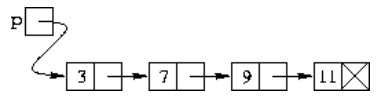
\includegraphics[width=0.6\textwidth]{Images/Linked1.png}
    \centering
    \caption{Lista singolarmente concatenata}
    \label{fig: Linked1}
\end{figure}

\footnote{Fonte dell'immagine: \textit{https://www.science.unitn.it/~brunato/labpro1/lista.html}}

Nel codice, dove viene implementata una coda con priorità tramite lista concatenata, il dato è un valore che scandisce la priorità del nodo. La lista concatenata (classe \textit{LinkedListQueue} in figura \ref{fig: DiagrammaDelleClassi}) è stata realizzata implementando tutti i metodi che non erano stati scritti nella classe astratta \textit{Queue} e ogni nodo è rappresentato dalla classe \textit{LinkedListNode} in figura \ref{fig: DiagrammaDelleClassi}.

Questa struttura dati ha diversi vantaggi e svantaggi, che si qualificano in base all'efficienza che hanno nelle varie operazioni standard:

\begin{itemize}
    \item \verb|Inserimento di un valore in testa|: operazione velocissima con una complessità di $\Theta$(1).

    \begin{figure}[H]
    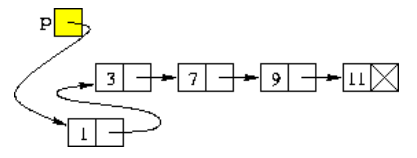
\includegraphics[width=0.5\textwidth]{Images/Linked2.png}
    \centering
    \caption{Inserimento in testa a una lista concatenata}
    \label{fig: Linked2}
    \end{figure}
    
    \footnote{Fonte dell'immagine: \textit{https://www.science.unitn.it/~brunato/labpro1/lista.html}}

    \item \verb|Rimozione di un valore|: in un caso generico di rimozione di un elemento con una certa chiave da una lista concatenata non ordinata (come si vede in figura \ref{fig: Linked3}), si devono seguire i seguenti passaggi:

    \begin{enumerate}
    
    \item Iniziare dal primo elemento della lista e confrontare la chiave dell'elemento con la chiave che deve essere rimossa.

    \item Se la chiave corrisponde, si può rimuovere l'elemento dalla lista aggiornando però i puntatori degli elementi precedenti e successivi all'elemento che vuoi rimuovere. Ad esempio, se l'elemento da rimuovere è il secondo in una lista, si deve impostare il puntatore del primo elemento al terzo elemento.
    
    \item Se la chiave non corrisponde, si passa all'elemento successivo nella lista e si ripete il passaggio 2.

    \item Continuare a seguire i passaggi 2 e 3 finché non si è controllato tutti gli elementi nella lista o fino a quando non si è trovato e rimosso l'elemento desiderato.
    
    \end{enumerate}

    Nella presente relazione, è necessario individuare ed estrarre il valore massimo all'interno di una coda con priorità implementata tramite una lista concatenata. Il valore massimo corrisponde all'elemento con il \emph{value} più elevato, ovvero con la priorità maggiore rispetto a tutti gli altri nodi. Poiché il valore massimo potrebbe trovarsi in qualsiasi posizione della lista, sia la sua ricerca che la sua rimozione richiedono un costo di $\Theta$(n). Ciò è dovuto al fatto che è necessario scorrere tutti e "n" gli elementi della lista. Inoltre, dopo la rimozione, sarà indispensabile aggiornare il campo \textit{next} del nodo precedente, assegnandogli il valore del campo \textit{next} del nodo appena rimosso. 

    \begin{figure}[H]
    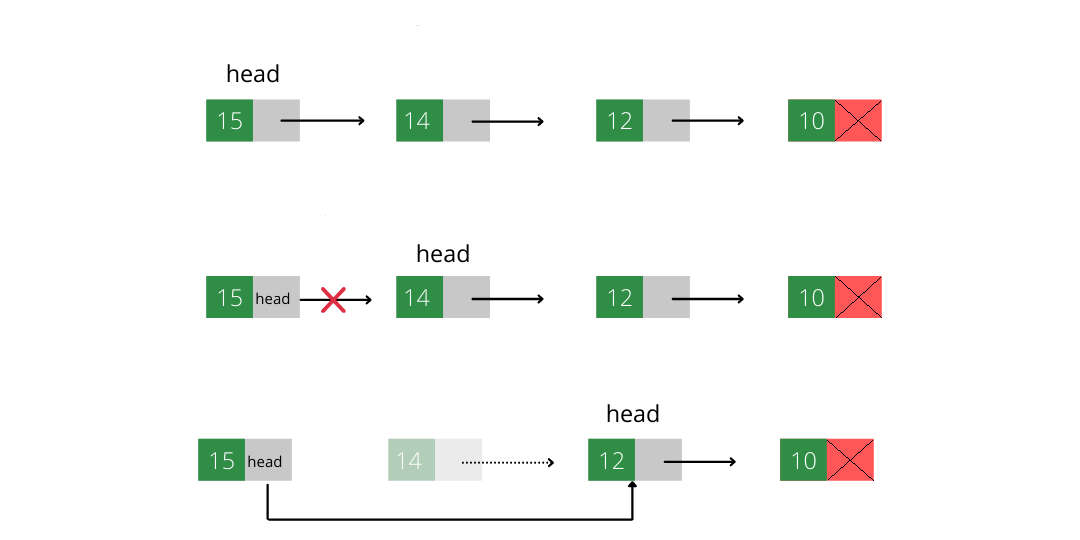
\includegraphics[width=0.9\textwidth]{Images/Linked3.png}
    \centering
    \caption{Cancellazione del secondo elemento da una lista concatenata}
    \label{fig: Linked3}
    \end{figure}
    
    \footnote{Fonte dell'immagine: \textit{https://www.geeksforgeeks.org/deletion-in-linked-list/}}

\end{itemize}

\subsubsection{Lista concatenata ordinata}
Una lista concatenata ordinata (nel codice è la classe \textit{SortedLinkedList} che eredita da \textit{LinkedList} come si vede dala figura \ref{fig: DiagrammaDelleClassi}) è analoga alla lista concatenata descritta precedentemente con la sola differenza che i valori sono ordinati in senso decrescente (nel caso di questa relazione e quindi di una scelta implementativa).

Analizziamo dunque le differenze implementative delle operazioni di inserimento e cancellazione:

\begin{itemize}
    \item \verb|Inserimento di un valore|: non sarà sufficiente inserire il nuovo nodo a inizio lista, bensì sarà necessario scorrere la lista finchè non si trova la posizione corretta in cui andrà inserito. Il caso peggiore è quando l'elemento da inserire è più piccolo di tutti gli altri nodi della lista e duqnue si dovrà posizionare in fondo ad essa (vedi figura \ref{fig: Linked4}). Il costo dunque è di $O(n)$.

    \begin{figure}[H]
    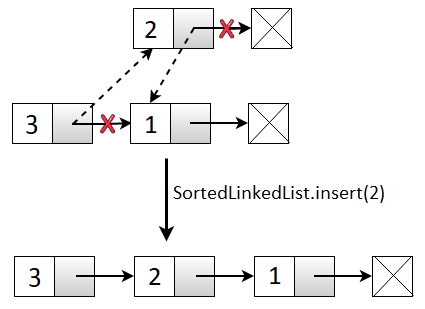
\includegraphics[width=0.6\textwidth]{Images/Linked4.png}
    \centering
    \caption{Inserimento di un elemento in una lista ordinata}
    \label{fig: Linked4}
    \end{figure}
    
    \footnote{Fonte dell'immagine: \textit{https://www.techiedelight.com/sorted-insert-in-linked-list/}}


    \item \verb|Rimozione del valore massimo|: in questo caso, l'operazione è molto agevolata dal fatto che la lista è ordinata in senseo decrescente. Per questo motivo, basterà modificare la testa della lista per rimuovere l'elemento massimo. Quest'operazione avrà dunque una complessità pari a $\Theta$(1). Vedi figura \ref{fig: Linked5}

    \begin{figure}[H]
    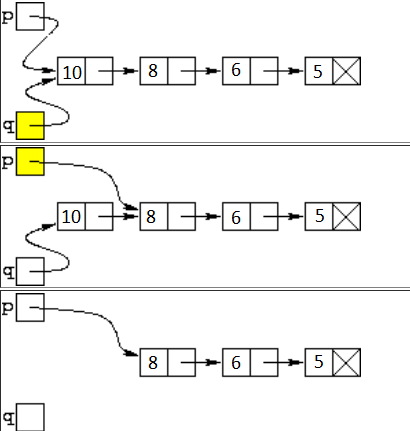
\includegraphics[width=0.4\textwidth]{Images/Linked5.png}
    \centering
    \caption{Cancellazione del primo elemento da una lista ordinata}
    \label{fig: Linked5}
    \end{figure}
    
    \footnote{Fonte dell'immagine: \textit{https://www.science.unitn.it/~brunato/labpro1/lista.html}}

\end{itemize}

\clearpage

\subsection{Prestazioni teoriche volute}

Come accennato in precedenza, questa relazione confronta le prestazioni di tre operazioni su una coda di priorità, che sono state implementate utilizzando tre diverse strutture dati. Le operazioni prese in considerazione sono l'inserimento di nuovi valori, la ricerca del valore massimo e l'estrazione di tale valore.

\subsubsection{Inserimento dei valori}

    \begin{enumerate}
    
    \item Per inserire un valore in un max heap, viene aggiunto un nuovo nodo nell'ultimo livello con un valore di $-\infty$, questo avviene in tempo costante. Successivamente, tramite l'utilizzo di \textit{increaseKey(i, key)}, viene impostato il valore del nodo, garantendo il mantenimento delle proprietà del max heap. La complessità dell'inserimento è quindi di $O(\log_2(n))$.
    
    \item In una lista concatenata non ordinata, l'inserimento avviene sempre in testa, rendendo la complessità dell'inserimento $\Theta(1)$.
    
    \item In una lista concatenata ordinata, è necessario scorrere gli elementi della lista fino a trovare la posizione corretta del nuovo valore. Nel caso migliore, l'inserimento avviene in testa, mentre nel caso peggiore l'elemento viene inserito alla fine della lista dopo aver attraversato tutti gli n elementi. Di conseguenza, la complessità dell'inserimento sarà $O(n)$.
    
    \end{enumerate}

\subsubsection{Ricerca del valore massimo}

    \begin{enumerate}
    
    \item In un max heap, l'elemento con il valore massimo si trova nella radice dell'albero, nella posizione $0$ della lista memorizzata. La complessità per la ricerca del massimo è quindi $\Theta(1)$.
    
    \item In una lista concatenata non ordinata, gli elementi non seguono un ordine specifico. Quindi, per trovare il nodo con il valore massimo è necessario scorrere tutti i valori. La complessità di questa operazione è quindi $\Theta(n)$.
    
    \item In una lista concatenata ordinata, poiché i valori sono ordinati in modo decrescente, l'elemento con il valore massimo si troverà nella prima posizione, ovvero all'inizio della lista (i.e \textit{head}). L'accesso a questo elemento avverrà in tempo costante, con una complessità di $\Theta(1)$.
    
    \end{enumerate}

\subsubsection{Estrazione del valore massimo}

    \begin{enumerate}
    
    \item Nel max heap, per estrarre il valore massimo, è necessario rimuovere l'elemento inziale. Per garantire che il max heap mantenga le sue proprietà, l'elemento iniziale viene sostituito con l'ultimo elemento della lista memorizzata (foglia). Successivamente, viene chiamato il metodo \textit{maxHeapify(0)}, che riorganizza l'albero in modo che rimanga un max heap. Poiché la foglia inserita come radice scenderà nell'albero di un livello alla volta fino a quando l'albero non sarà nuovamente un max heap, il costo di questa operazione è $O(\log_2(n))$ ($\log_2(n)$ corrisponde al numero massimo di livello presenti nell'albero).
    
    \item In una lista concatenata non ordinata, una volta individuato il valore da rimuovere, questo viene scollegato dalla lista come mostrato nella figura \ref{fig: Linked3}. Il caso peggiore ha complessità di questa operazione è $\Theta(n)$ (come la ricerca del massimo).
    
    \item In una lista concatenata ordinata il costo della rimozione è costante ($\Theta(1)$) (uguale alla ricerca) in quanto è sufficiente aggiornare il primo elemento (ovvero \textit{head}) della lista.
    
    \end{enumerate}

\subsubsection{Tabella riassuntiva}

\begin{table}[ht]
  \centering
  \begin{tabular}{cccc}
    \toprule
    Struttura dati & Inserimento & Ricerca del massimo & Estrazione del massimo \\
    \midrule
    Max heap & $O(\log_2(n))$ & $\Theta(1)$ & $O(\log_2(n))$   \\
    \hdashline
    Lista concatenata & $\Theta(1)$ & $\Theta(n)$ & $\Theta(n)$   \\
    \hdashline
    Lista concatenata ordinata & $O(n)$ & $\Theta(1)$ & $\Theta(1)$  \\
    \bottomrule
  \end{tabular}
    \caption{Prestazioni attese delle varie operazioni}
    \label{tab:Prestazioni}
\end{table}

\clearpage

\section{Descrizione degli esperimenti condotti}
Per ogni implementazione della coda con priorità, si sono condotti test su ogni funzione (inserimento dei valori, ricerca ed estrazione del massimo) utilizzando un incremento graduale di valori (\textit{n}), da 1 fino a 600, con uno step di 30 unità ad ogni iterazione. 

In totale sono stati effettuati dunque 20 test (corrispondono alla prima colonna delle tabelle in sezione \ref{sec:tabelleTempi}).

Al fine di ottenere risultati più affidabili, ciascun test è stato eseguito 100 volte e i tempi di esecuzione sono stati mediati. In tal modo si è ridotta l'influenza di altri processi in esecuzione sulla macchina durante i test. Per misurare i tempi di esecuzione, è stato utilizzato il metodo \textit{timeit(stmt, number)} del modulo Python \textit{timeit}. Il primo parametro (\emph{stmt}) corrisponde alla funzione da eseguire, mentre il secondo parametro (\emph{number}) indica il numero di iterazioni da fare. Questo metodo restituisce il tempo totale impiegato per l'esecuzione dei test.

\subsection{Operazioni effettuate su una copia della coda con priorità}
\textbf{Nota bene:}  I test vengono eseguiti su una copia della coda fornita come parametro. Ciò è necessario poiché tali test coinvolgono ripetute operazioni che modificano la struttura della lista. Senza l'uso di una copia, ogni operazione influenzerebbe la lista rispetto all'iterazione precedente, portando a risultati di test errati.

Per questo motivo viene utilizzata la libreria \verb|copy| e la sua funzione \textit{copy.deepcopy()}, come descritto in sezione \ref{sec:usoLibrerie}.

\clearpage

\section{Tabelle dei tempi di esecuzione}

\label{sec:tabelleTempi}

Di seguito sono presentate le tabelle che mostrano i tempi di esecuzione delle tre operazioni (inserimento, ricerca ed estrazione del massimo) eseguite sulla coda con priorità.

\begin{figure}[H]
    \centering
    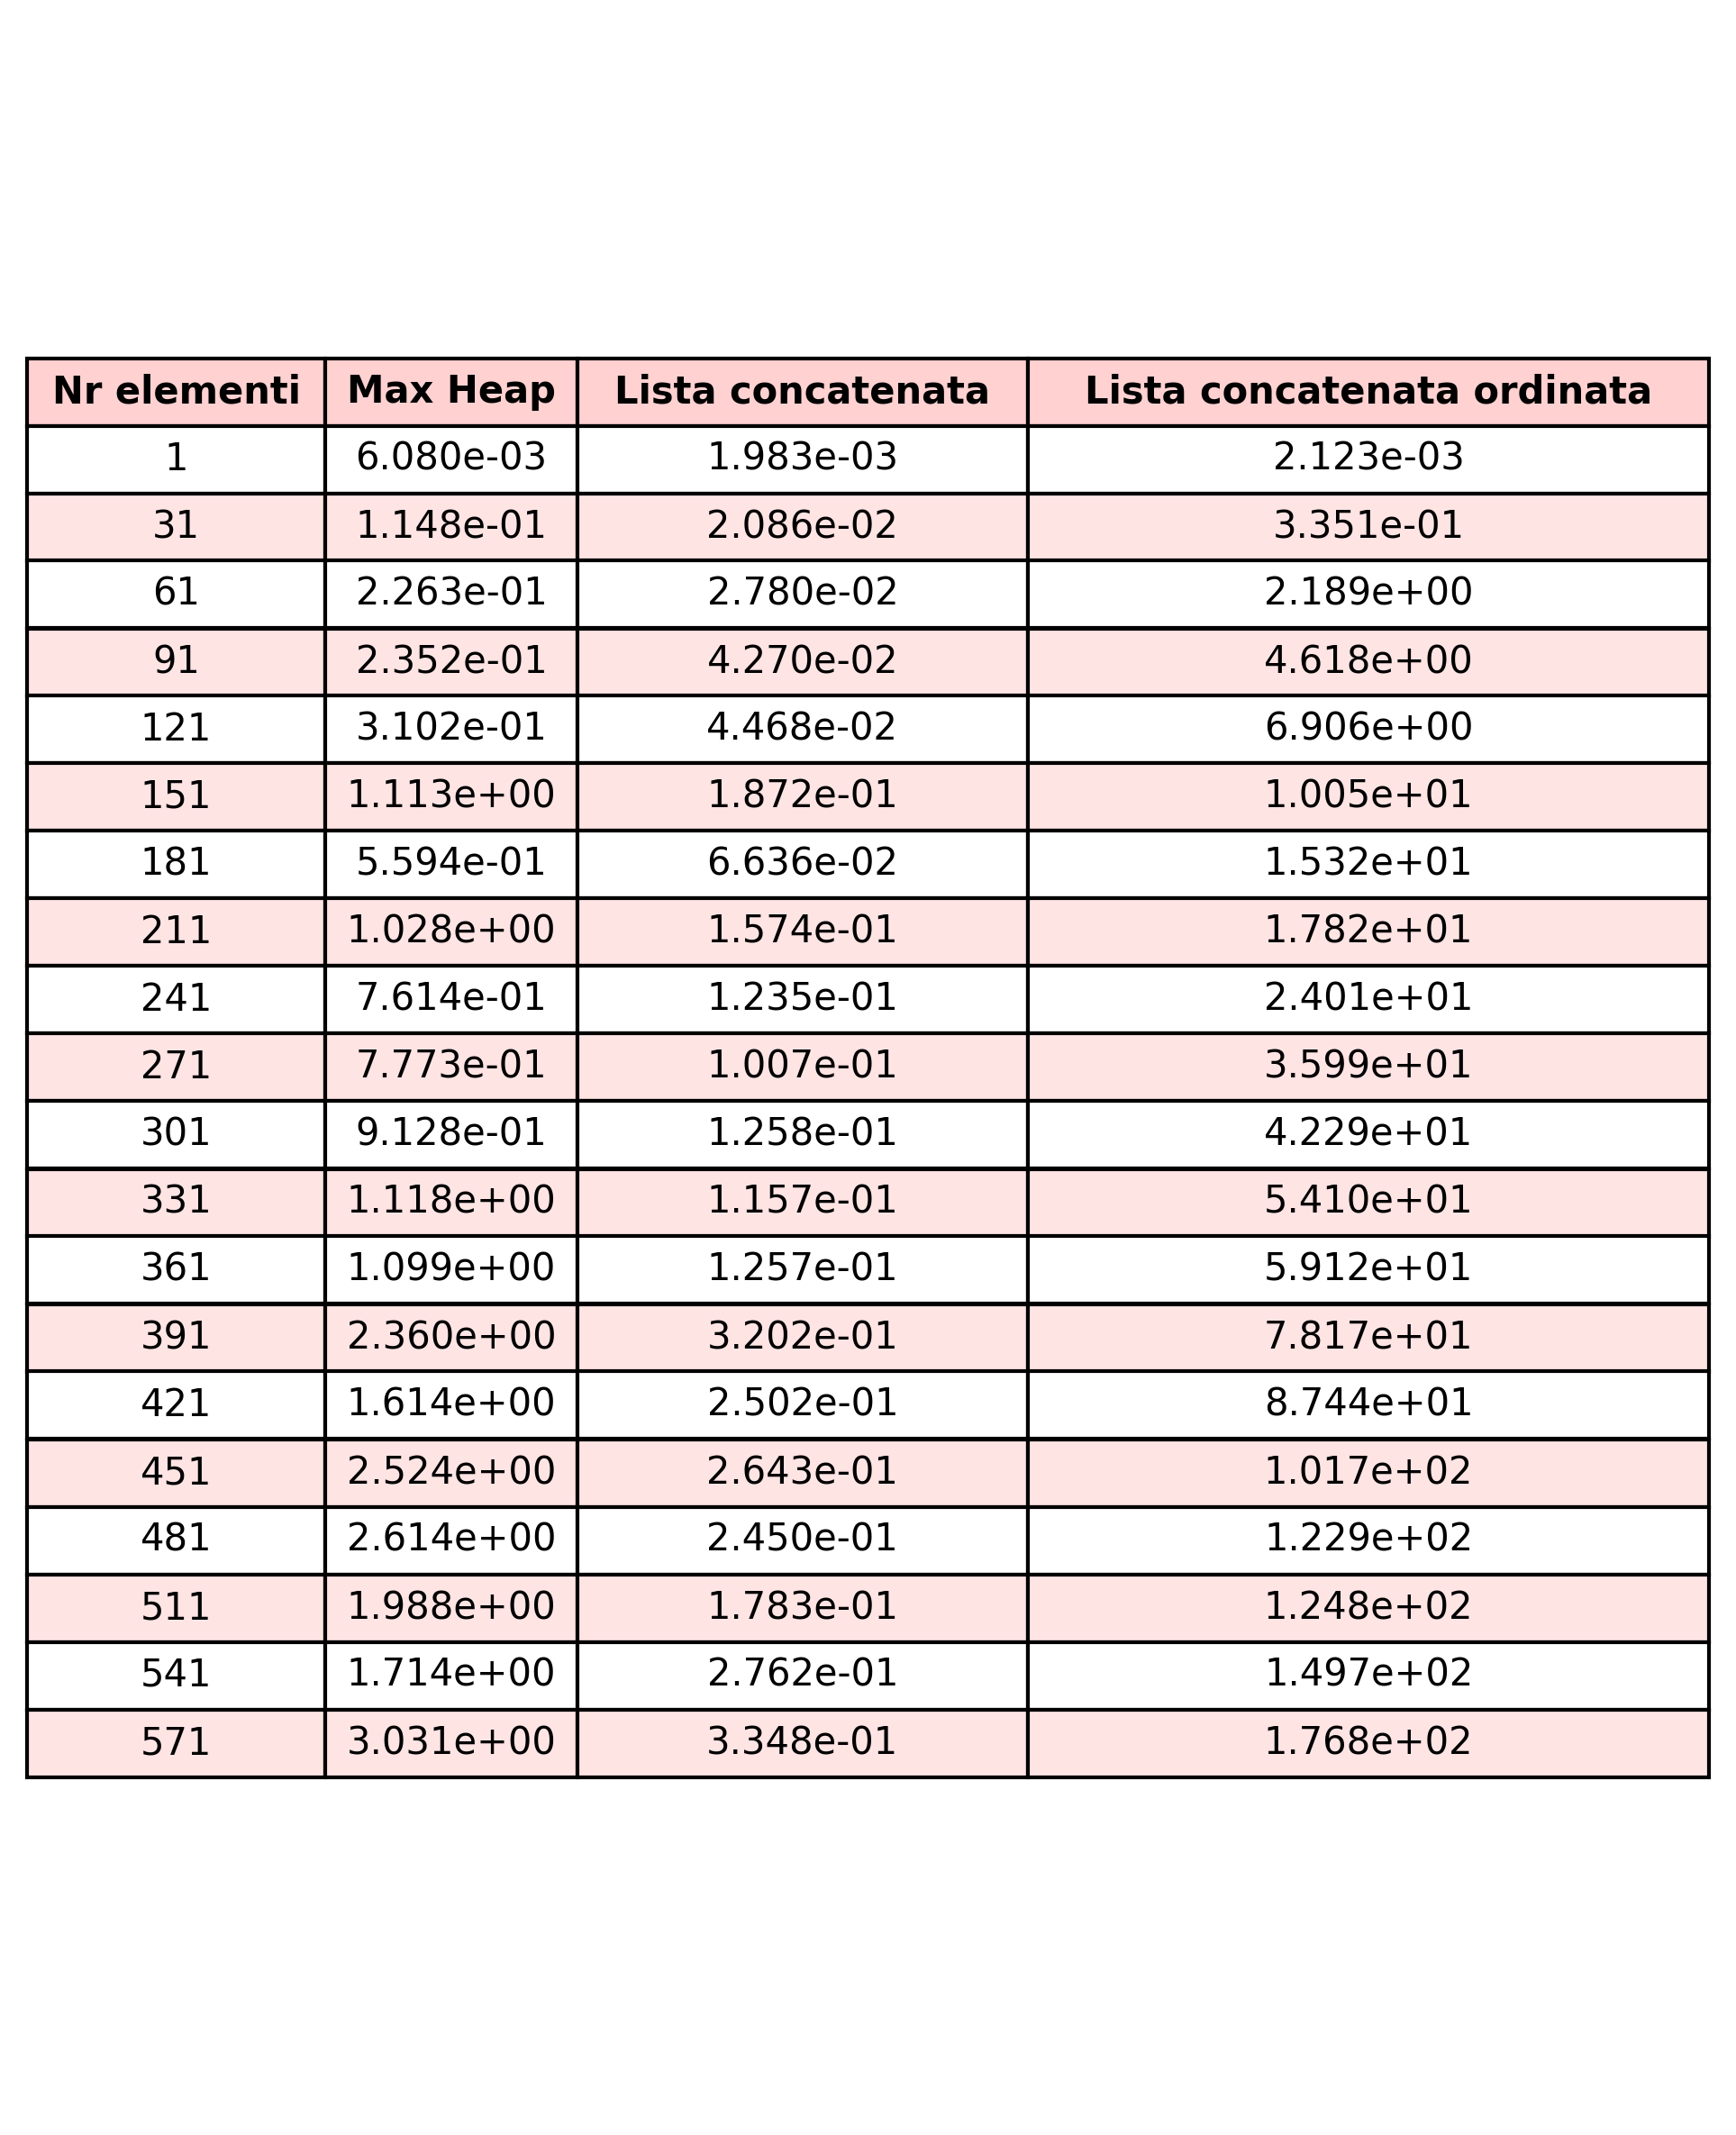
\includegraphics[width=\textwidth]{Images/TempoInserimento.png}
    \caption{Tempi d'esecuzione dell'inserimento di "n" valori nella coda [mS]}
    \label{fig:TabellaInserimento}
\end{figure}

\begin{figure}[h]
    \centering
    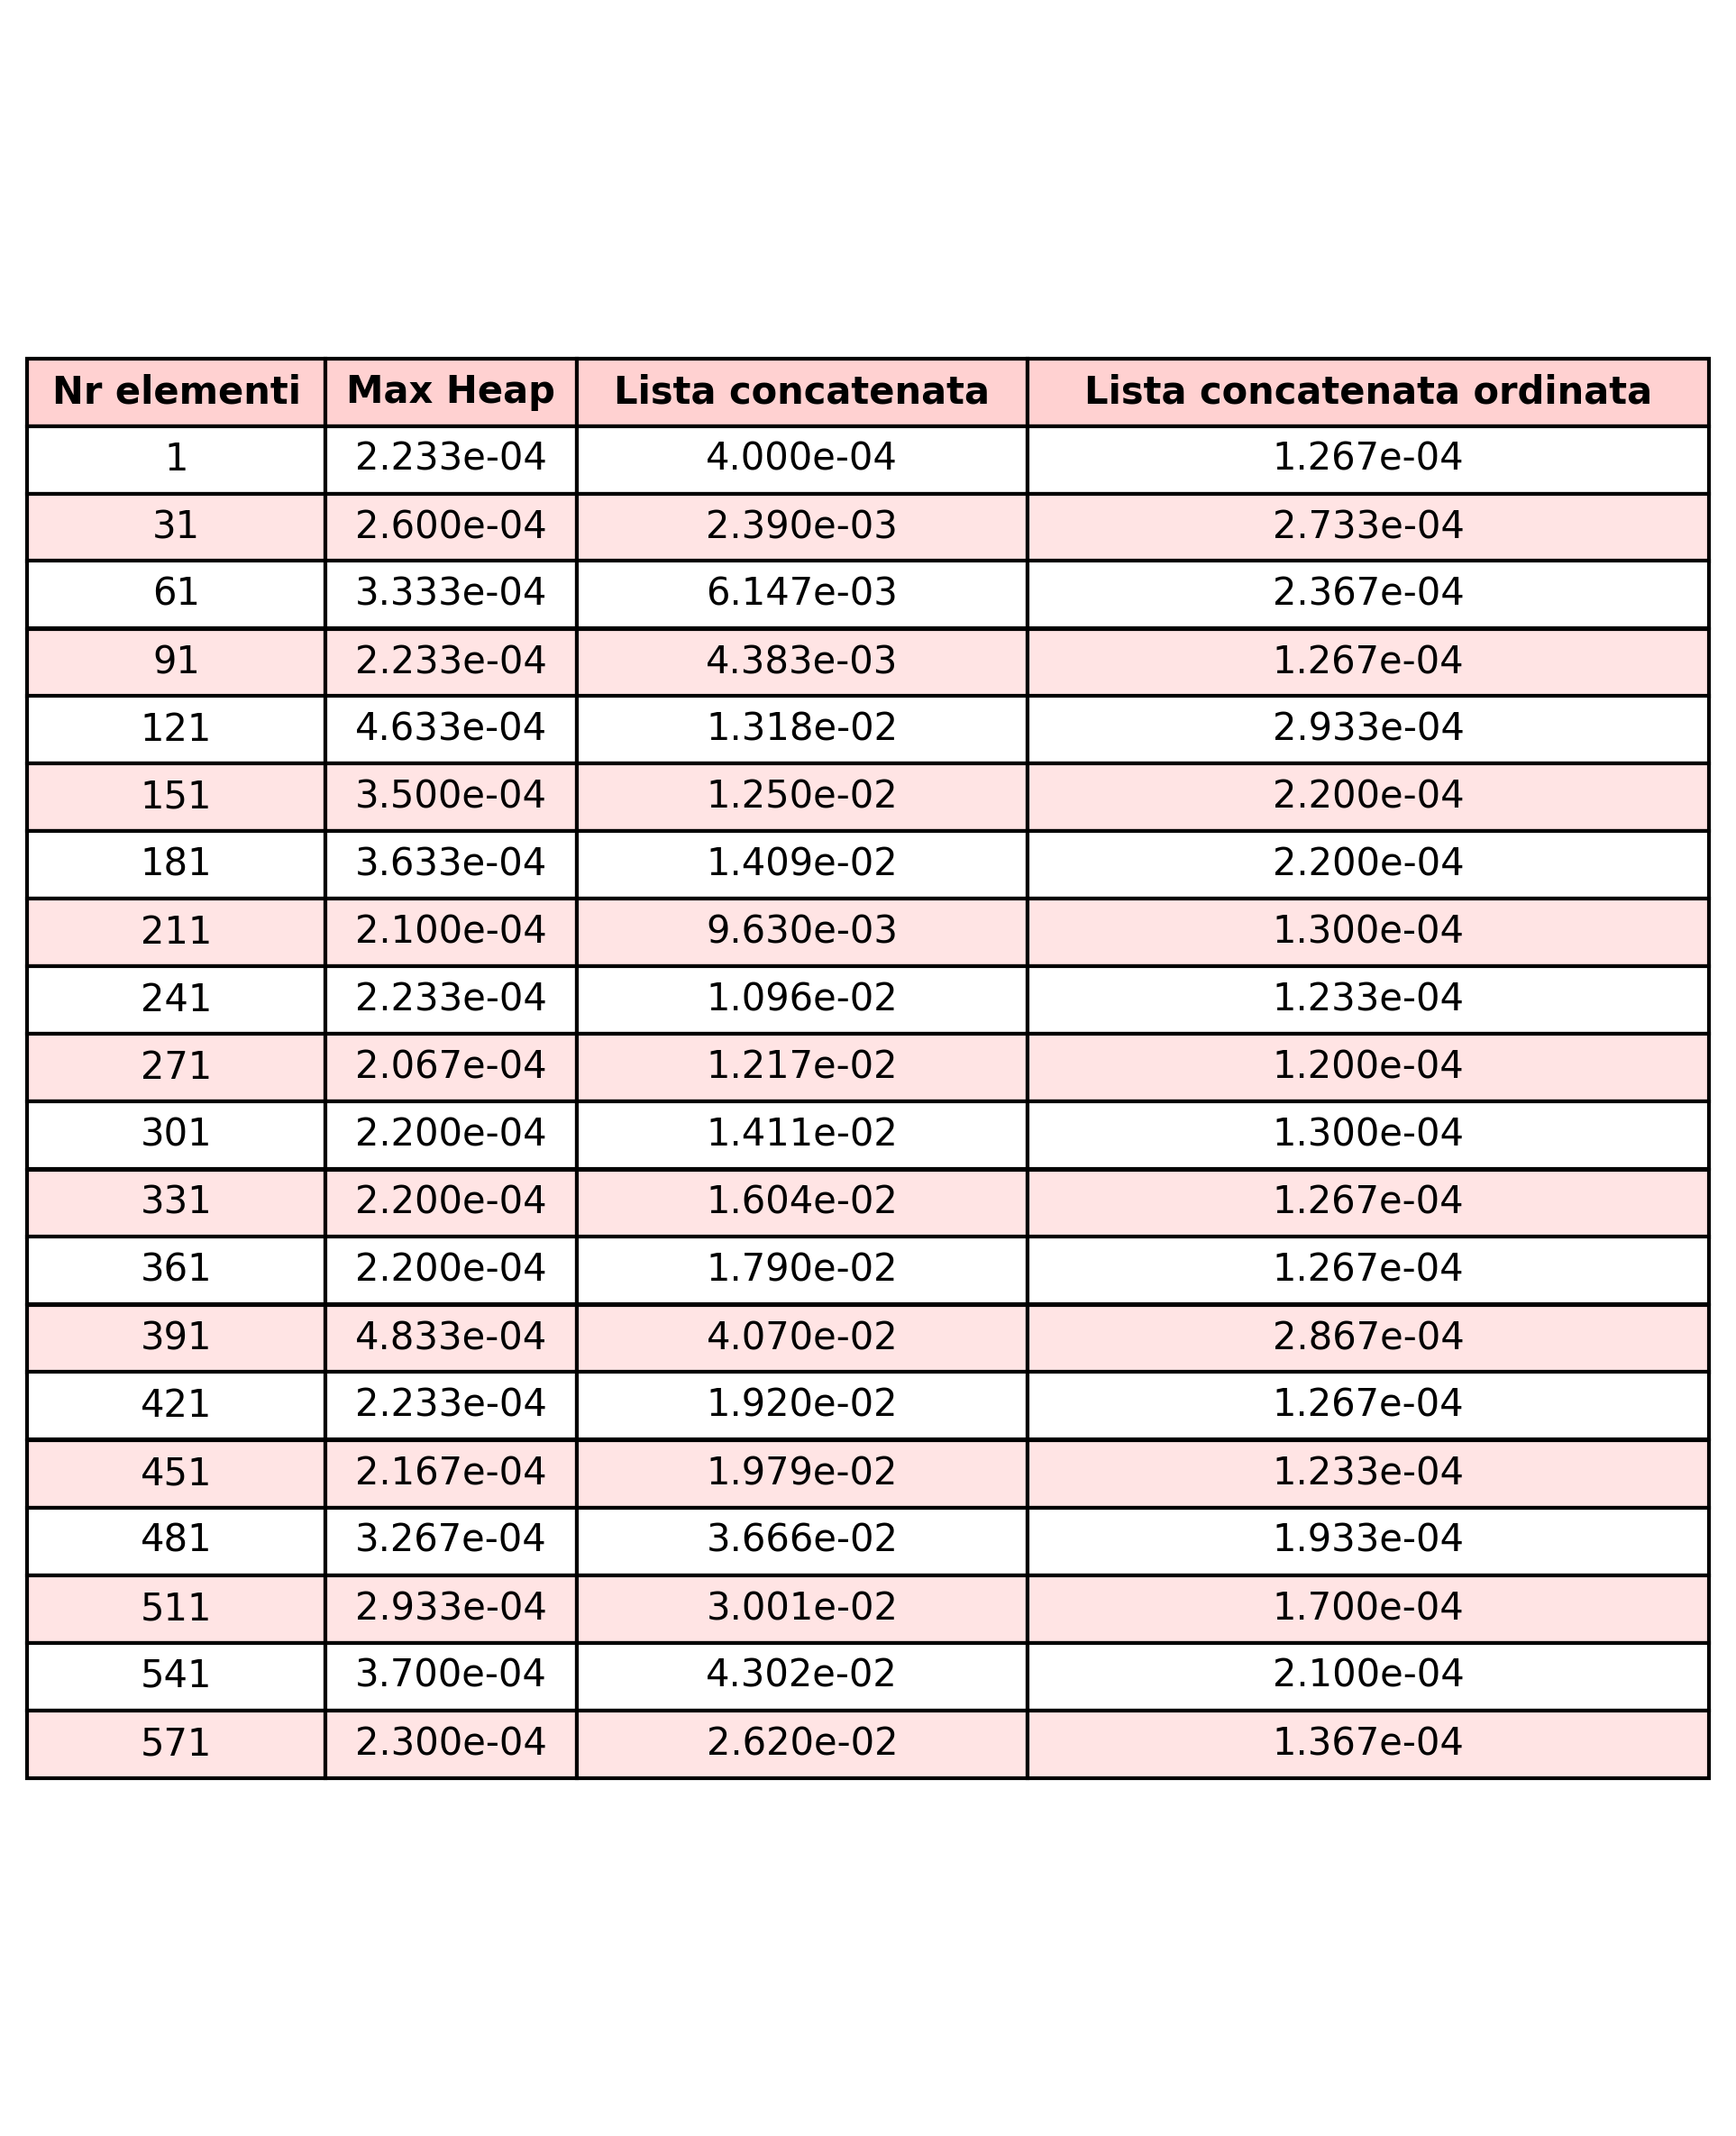
\includegraphics[width=\textwidth]{Images/TempoRicercaMassimo.png}
    \caption{Tempi d'esecuzione della ricerca del valore massimo da una coda di "n" elementi [mS]}
    \label{fig:TabellaRicerca}
\end{figure}

\begin{figure}[h]
    \centering
    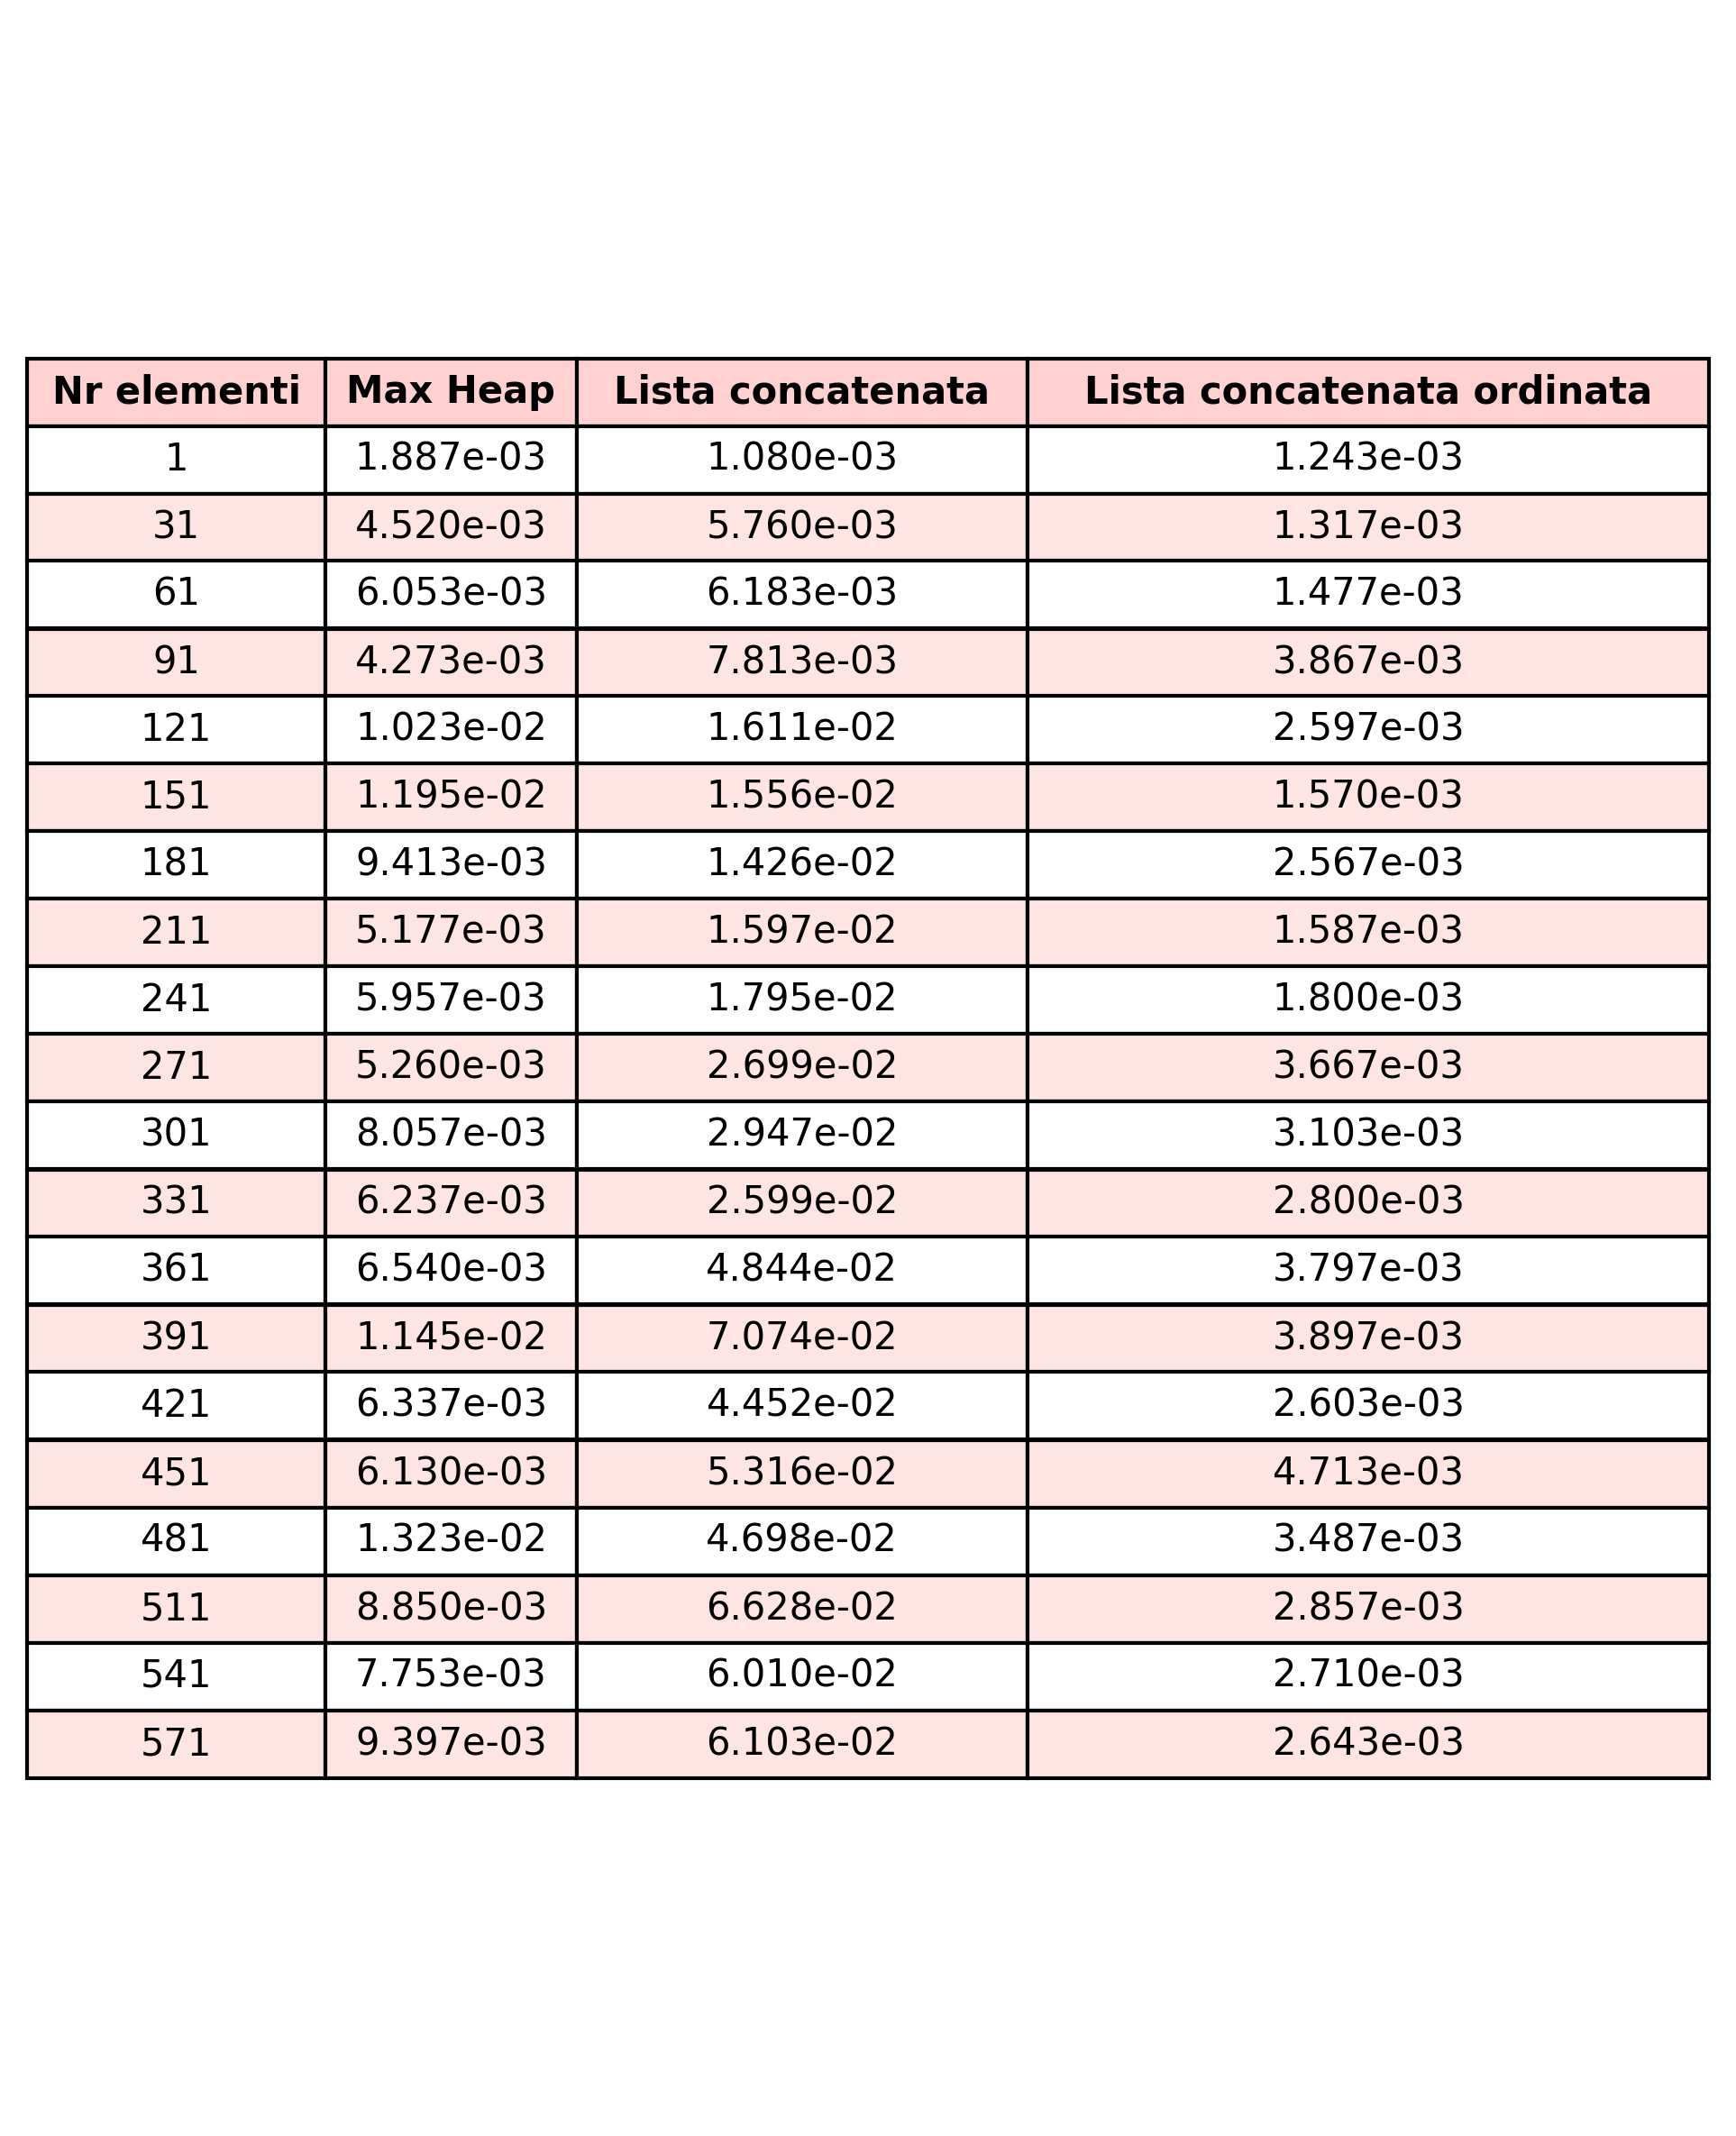
\includegraphics[width=\textwidth]{Images/TempoEstMassimo.png}
    \caption{Tempi d'esecuzione dell'estrazione del valore massimo da una coda di "n" elementi [mS]}
    \label{fig:TabellaEstrazione}
\end{figure}

\clearpage

\section{Grafici dei tempi di esecuzione}

\label{sec:grafici}

Di seguito sono presentati i grafici che consentono di confrontare le prestazioni misurate delle diverse implementazioni della coda con priorità.
I grafici illustrano la variazione del tempo di esecuzione delle tre funzioni implementate della coda con priorità (tutto ciò al variare del numero di elementi presenti nella coda).

\begin{figure}[H]
    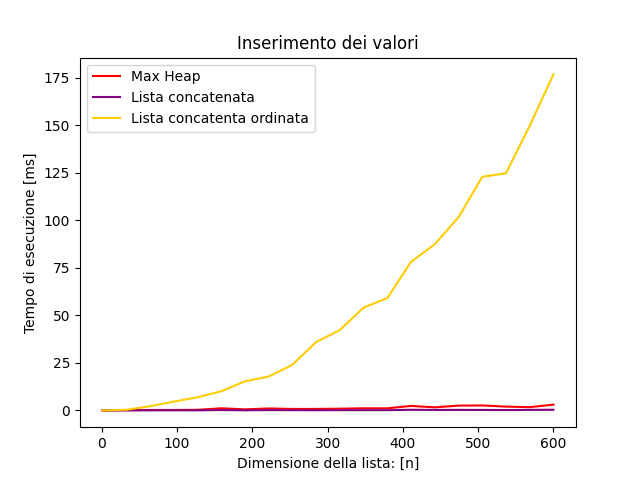
\includegraphics[width=\textwidth]{Images/GraficoInserimento.png}
    \centering
    \caption{Tempi di esecuzione dell'inserimento di n valori nella coda}
    \label{fig:GraficoInserimento}
\end{figure}

\begin{figure}[h]
    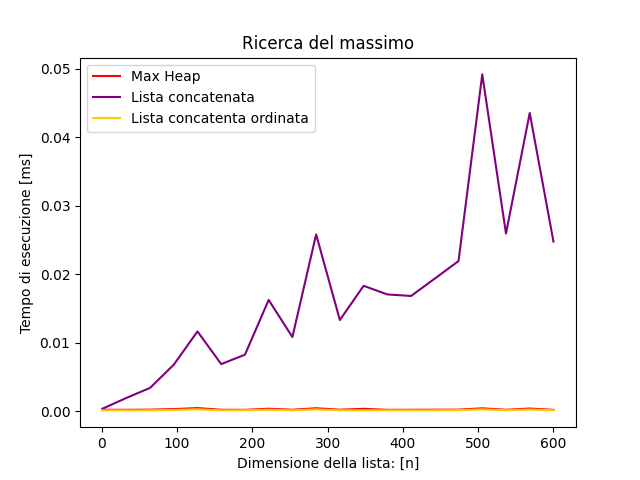
\includegraphics[width=\textwidth]{Images/GraficoRicercaMassimo.png}
    \centering
    \caption{Tempi d'esecuzione della ricerca del valore massimo al variare del numero di elementi presenti nella coda}
    \label{fig:GraficoRicerca}
\end{figure}

\begin{figure}[h]
    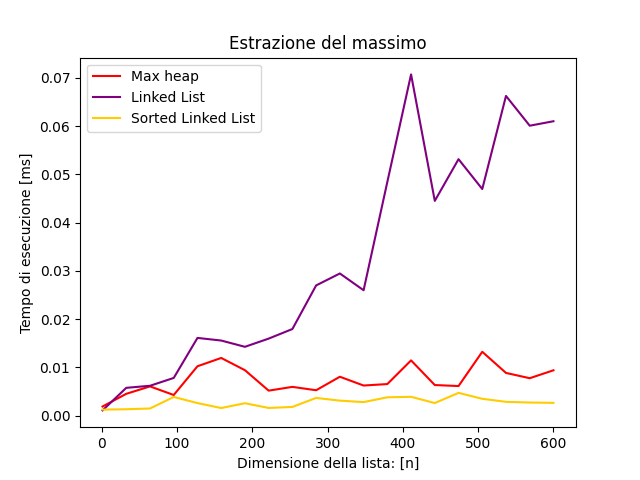
\includegraphics[width=\textwidth]{Images/GraficoEstMassimo.png}
    \centering
    \caption{Tempi d'esecuzione dell'estrazione del valore massimo al variare del numero di elementi presenti nella coda}
    \label{fig:GraficoEstrazione}
\end{figure}

\clearpage

\section{Analisi e osservazioni sui risultati finali}

In questa sezione finale viene presentata un'analisi dettagliata delle prestazioni delle tre operazioni per le tre diverse implementazioni della coda con priorità, utilizzando le tabelle e i grafici prodotti precedentemente come supporto visivo. Il presente capitolo si propone di analizzare in modo più approfondito i risultati ottenuti e di trarre osservazioni significative da essi. L'obiettivo finale di questa sezione è quello di offrire una sintesi completa delle osservazioni tratte dai risultati finali dell'analisi, mettendo in luce le caratteristiche e le differenze significative tra le tre implementazioni della coda con priorità (vedere tabella riassuntiva \ref{tab:Prestazioni}).

\subsection{Inserimento dei valori}

La tabella rappresentata nella figura \ref{fig:TabellaInserimento} riporta i tempi di esecuzione dell'operazione di inserimento nelle diverse implementazioni della coda con priorità. Sulla base di questi valori, è stato generato il grafico illustrato nella figura \ref{fig:GraficoInserimento}, che offre una rappresentazione visiva della complessità dell'operazione di inserimento:

\begin{itemize}
\item Fare riferimento alla tabella \ref{fig:TabellaInserimento} e al conseguente grafico \ref{fig:GraficoInserimento}.

\item L'inserimento in un max heap ha un costo con una complessità pari a $O(\log_2(n))$. Pertanto, in termini di prestazioni, si posiziona a metà strada rispetto alle altre due implementazioni (\ref{fig:GraficoInserimento}).

\item L'inserimento in una lista concatenata non ordinata ha un costo costante ($\Theta(1)$), il che significa che i tempi di esecuzione sono notevolmente inferiori rispetto alle altre due implementazioni. Questo perché l'inserimento viene effettuato in testa alla coda, senza richiedere operazioni di ricerca o riorganizzazione dei dati.

\item L'inserimento in una lista concatenata ordinata è un'operazione molto costosa. Dall'andamento rappresentato nel grafico (linea gialla), è evidente che i tempi di esecuzione aumentano linearmente all'aumentare del numero di valori nella lista. Ciò è dovuto al fatto che i valori sono ordinati, e nel caso peggiore (valore da inserire maggiore di tutti gli altri), è necessario scorrere l'intera lista per trovare la posizione corretta di inserimento. Il costo di questa operazione cresce in modo più significativo rispetto all'implementazione basata sul max heap (complessità $O(n)$, $O$ e non $\Theta$ in quanto non è detto che scorra tutta la lista).

\end{itemize}

\subsection{Ricerca del valore massimo}

\begin{itemize}
\item Fare riferimento alla tabella \ref{fig:TabellaRicerca} e al conseguente grafico \ref{fig:GraficoRicerca}.

\item La ricerca del valore massimo in una coda con priorità implementata tramite un max heap ha un costo costante (complessità $\Theta(1)$) grazie alla sua struttura. Questo è evidente dal grafico \ref{fig:GraficoRicerca}, in quanto la linea rossa e la linea gialla (corrispondenti alla lista concatenata ordinata) si sovrappongono approssimativamente e rimangono costanti all'aumentare delle dimensioni della coda.

\item La ricerca del valore massimo in una lista concatenata non ordinata è un'operazione molto costosa. Questo è dovuto al fatto che, essendo la lista non ordinata, è necessario scorrere tutti gli elementi al suo interno (complessità $\Theta(n)$). Come previsto dalla teoria, il tempo di esecuzione dell'algoritmo aumenta linearmente con la dimensione (n) della lista.

\item Per la lista concatenata ordinata vale lo stesso principio del max heap. Grazie alla sua struttura, è sufficiente accedere a uno dei due estremi della coda (direttamente tramite l'head o la tail, a seconda dell'ordine della lista) per trovare il valore massimo (complessità $\Theta(1)$).

\end{itemize}

\subsection{Estrazione del valore massimo}

\begin{itemize}
\item Fare riferimento alla tabella \ref{fig:TabellaEstrazione} e al conseguente grafico \ref{fig:GraficoEstrazione}.

\item L'estrazione del valore massimo in un max heap ha un costo con complessità $O(\log_2(n))$. Questo è dovuto al fatto che una volta che viene rimosso l'elemento massimo (che corrisponde alla radice), è necessario eseguire una serie di operazioni per ripristinare e mantenere le proprietà del max heap. Tali operazioni hanno un costo logaritmico.

\item Allo stesso modo della ricerca del valore massimo, nell'estrazione del massimo da una lista concatenata, il costo aumenta linearmente all'aumentare della dimensione della lista.

\item L'estrazione del massimo in una lista concatenata ordinata ha un costo costante, che rimane invariato rispetto alla ricerca del massimo nella stessa struttura dati.

\end{itemize}

\subsection{Conclusioni}


L'analisi teorica della complessità degli algoritmi è stata validata attraverso test e misurazioni sperimentali, confermando le previsioni. I risultati ottenuti evidenziano le diverse prestazioni delle implementazioni considerate per le operazioni di inserimento di un valore generico, ricerca ed estrazione del valore massimo.

La lista concatenata non ordinata si distingue per la velocità nell'inserimento, ma presenta limitazioni nella ricerca ed estrazione del valore massimo, che richiedono un tempo proporzionale alla dimensione della lista. D'altra parte, la lista concatenata ordinata offre una ricerca del valore massimo rapida, ma a scapito di un inserimento più lento.

Il max heap rappresenta un compromesso tra le due strutture dati precedenti. Entrambi l'inserimento e l'estrazione del massimo hanno una complessità logaritmica, garantendo buone prestazioni in situazioni con un grande numero di elementi. Inoltre, la ricerca del valore massimo avviene in tempo costante, contribuendo alla sua efficienza complessiva.

In conclusione, la scelta della struttura dati dipende dalle specifiche esigenze dell'applicazione. La lista concatenata può essere preferita in scenari in cui l'inserimento è prioritario, ma si può accettare un'efficienza leggermente inferiore nella ricerca ed estrazione del massimo. Al contrario, se la ricerca del massimo è frequente e si richiede un buon compromesso tra operazioni di inserimento ed estrazione, il max heap si rivela una scelta più appropriata.

\end{document}

